\chapter{Microbolómetros y descripción de especificaciones}
Un microbolómetro es un elemento resistivo fabricado con un material de baja capacidad térmica y alto coeficiente de temperatura, lo que permite que la radiación absorbida provoque un cambio significativo en su resistencia. El dispositivo opera mediante una corriente o voltaje de polarización controlada que atraviesa el detector mientras se monitorea el voltaje o corriente de salida. En este proceso, la energía radiante genera calor en el material, lo que altera la resistencia, sin interacción directa entre fotones y electrones.


El astrónomo S.P. Langley diseñó el primer bolómetro en 1880, utilizando platino ennegrecido como material absorbente y un puente de Wheatstone como circuito de detección. La tecnología moderna de bolómetros comenzó en los años 1980 con los avances de Honeywell en óxido de vanadio (VOx) y de Texas Instruments en silicio amorfo (a-Si). Mucho de este desarrollo ocurrió bajo proyectos militares clasificados en Estados Unidos, por lo que la divulgación de esta información a la comunidad científica data desde 1992.


Es muy difícil tener una representación exacta de un microbolómetro, pero este se puede representar como un circuito divisor de voltaje (Figura \ref{fig:voltage_divider}). Si el circuito está abierto y no hay radiación presente, el microbolómetro se encontrará a temperatura ambiente $T_{0}$, si el circuito está cerrado, la corriente fluirá y la resistencia del microbolómetro, $R_{B}$, se calentará, esto provocará que la temperatura incremente a $T_{1}$. Si ahora la radiación cae sobre el microbolómetro, la temperatura cambiará en un factor de $\Delta T$. Esto causará una modificación en la resistencia del microbolómetro, lo que a su vez generará una variación en el voltaje ($V_{RL}$) a través de la resistencia de carga $R_{L}$ \cite{Rogalski}. 

            \begin{figure}[hbtp]
                \centering
                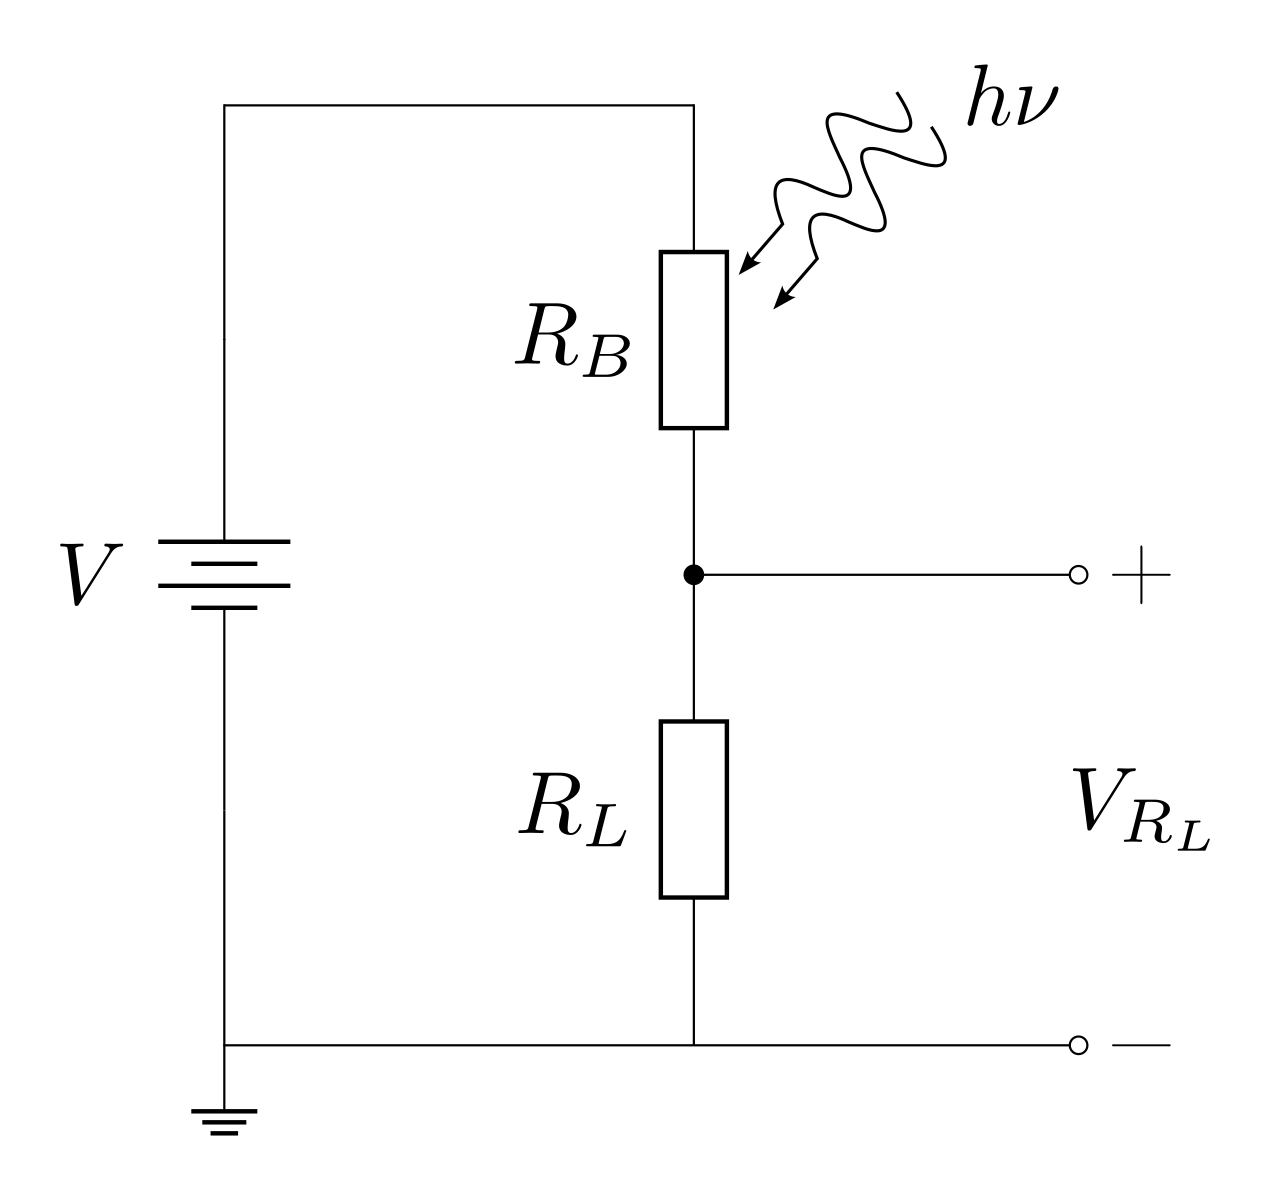
\includegraphics[width=0.5\textwidth]{voltage_divider}
                \caption{Representación de un microbolómetro como circuito eléctrico}
                \label{fig:voltage_divider}
            \end{figure} 

\section{Diseño de un arreglo de microbolómetros}
El diseño de un microbolómetro generalmente incluye un material absorbedor y un material que funge como termómetro, lo que lleva a un incremento de la temperatura debido a la absorción de radiación infrarroja, provocando finalmente un cambio en la resistencia de sus elementos. La variación en la resistencia se transmite eléctricamente al circuito integrado de lectura (ROIC) para su posterior procesamiento. Para aumentar la sensibilidad, el termómetro se mantiene aislado térmicamente del sustrato del ROIC \cite{Bhan2009}.

El diagrama esquemático de la estructura típica de un microbolómetro se muestra en la Figura \ref{fig:ubol sch}.
            \begin{figure}[hbtp]
                \centering
                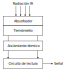
\includegraphics[width=0.4\textwidth]{ubol_sch}
                \caption{Diagrama esquemático de un microbolómetro}
                \label{fig:ubol sch}
            \end{figure}
\newpage
Un píxel en un arreglo de microbolómetros puede tener un área que varía entre $15\times 15 \mu m^{2}$ y $55\times 55 \mu m^{2}$. La estructura de un pixel, mostrada en la Figura, generalmente es descrita como un \textit{puente}, el cual se trata de una membrana suspendida que incluye una capa absorbente para la radiación infrarroja y un elemento termosensible que transforma el cambio de temperatura de la membrana en una señal eléctrica de salida. El \textit{piso} de este \textit{puente} es un circuito de lectura unitario y las dos \textit{rampas} son brazos de soporte utilizados para la conexión eléctrica, estos ayudan a mejorar el aislamiento térmico \cite{Vincent}, \cite{Budzier}.


Para un microbolómetro es esencial contar con una temperatura estable, esto con la finalidad de tener una mejor detección de radiación infrarroja. El vacío provee un buen aislamiento térmico, debido a que la pérdida de calor por conducción o convección es mínima. Mientras más vacío se tenga en el envase del detector mejor será la eficiencia \cite{Lau2010}.
Generalmente el microbolómetro requiere una atmósfera de vacío menor a 1 Pa para aislar la transferencia de calor y mejorar su respuesta \cite{Liu2020}.


    \section{Propiedades}
    En esta sección se definirán algunas propiedades importantes que son utilizadas para caracterizar el desempeño de microbolómetros.
        \subsection{Responsividad}
        La responsividad ($R$) se refiere a la capacidad que tiene un detector de convertir radiación incidente en una señal eléctrica
        \begin{equation}
        R = \frac{se\tilde{n}al\ de\ salida}{radiaci\acute{o}n\ de\ entrada}
        \label{eq:Responsivity}
        \end{equation}
        
        Para los microbolómetros, generalmente la radiación de entrada se define en términos de flujo radiante ($\Phi_{S}$), el cual es el producto de la irradiancia ($E$) por el área del detector ($A_{d}$) y la señal de salida  puede ser voltaje ($V_{S}$) o corriente ($I_{S}$).
        \begin{equation}
        R = \frac{S}{\Phi_{S}}
        \label{eq:Responsividad}
        \end{equation}
        
        La responsividad de voltaje $R_{V}$ se define como:
        \begin{equation}
        R_{V} = \frac{V_{S}}{EA_{d}}\phantom{abc} [V/W]
        \label{eq:Rv}
        \end{equation}
        
        La responsividad de corriente es:
        \begin{equation}
        R_{I} = \frac{I_{S}}{EA_{d}}\phantom{abc} [A/W]
        \label{eq:Ri}
        \end{equation}
        
        La responsividad es un parámetro crucial para un detector, ayuda a anticipar la sensibilidad del circuito de medición necesario para observar la salida esperada o a decidir el nivel de ganancia del amplificador requerido para amplificar la señal adecuadamente \cite{Vincent}, \cite{Budzier}.
        
        \subsection{Diferencia de temperatura equivalente al ruido}
        La diferencia de temperatura equivalente al ruido (Noise Equivalent Temperature Difference - $NETD$), indica el cambio mínimo de temperatura que un microbolómetro puede detectar, reflejando su capacidad para distinguir pequeñas diferencias en la radiación térmica. Un valor de $NETD$ más bajo significa mayor sensibilidad térmica \cite{Jimenez}, \cite{Budzier}.


El NETD generalmente es proporcionado por el fabricante.
        
        \subsection{Detectividad}
        La detectividad ($D$) es un parámetro utilizado para comparar el desempeño entre distintos detectores con diferentes tamaños. Mientras más elevada sea la detectividad, mejor será el detector.
        
        La detectividad se calcula de la siguiente manera:
        \begin{equation}
        D = \frac{R_{V} \sqrt{A\Delta f}}{V_{N}}\phantom{abc} [cm\sqrt{Hz}/W]
        \label{eq:Detectivity}
        \end{equation}
        Donde:
        
        
        $R_{V}$ - Responsividad de voltaje.
        
        
        $A$ - Área del detector.
        
        
        $\Delta F$ - Ancho de banda del ruido del detector.
        
        
        $V_{N}$ - Ruido total del detector.
        
        \cite{Vincent}, \cite{Jimenez}, \cite{Budzier}, \cite{Bhan2009}.
                
        \subsection{Conductancia térmica}
        La conductancia térmica ($G_{th}$) mide la facilidad con la que fluye el calor a través de un material. En el caso de un microbolómetro, cuantifica la velocidad a la que la energía térmica se transfiere del elemento detector a su entorno o al disipador de calor. La conductancia se puede obtener mediante la siguiente ecuación:
        \begin{equation}
        G_{th} = 2K\frac{A}{l}\phantom{abc} [W/K]
        \label{eq:Conductancia}
        \end{equation}   
        Donde:
        
        
        $K$ - Coeficiente de conductividad térmica del material de los brazos de soporte del microbolómetro.
        
        
        $A$ - Área transversal del brazo del detector.
        
        
        $l$ - Longitud del brazo.
        
        \cite{BlancoMDA}, \cite{Jimenez} \cite{Bhan2009}.        
        \subsection{Capacitancia térmica}
        La capacitancia térmica ($C_{th}$) determina cuánto calor puede almacenar el detector. Con la siguiente ecuación podemos calcularla.
        \begin{equation}
        C_{th} = c\rho v\phantom{abc} [J/K]
        \label{eq:Capacitancia}
        \end{equation} 
        Donde:
        
        
        $c$ - Calor específico del material.
        
        
        $\rho$ - Densidad del material con el que esté fabricado el pixel del microbolómetro.
        
         
        $v$ - Volumen de la membrana del microbolómetro.
        
        \cite{BlancoMDA}, \cite{Jimenez} \cite{Bhan2009}.
        
        \subsection{Coeficiente de temperatura de la resistencia}
        El coeficiente de temperatura de la resistencia (Thermal Coefficient of Resistance - $TCR$) se define como la variación de la resistencia del microbolómetro ($R_{B}$) debido al cambio de temperatura:
        \begin{equation}
        \alpha_{B} = TCR =\frac{1}{R_{B}}\frac{dR_{B}}{dT_{S}}
        \label{eq:TCR}
        \end{equation}
        El cambio en la resistencia del microbolómetro en función de la temperatura depende de si el material es un metal o un semiconductor \cite{Budzier}, \cite{Wei2015}.         


La clave para desarrollar microbolómetros altamente sensibles es tener un coeficiente de temperatura alto $\alpha$, una masa térmica muy baja $C_{th}$ y un excelente aislamiento térmico (baja conductancia térmica) $G_{th}$ \cite{Rogalski}.

\section{Circuitos de lectura para un microbolómetro}